\documentclass[tikz,border=10pt]{standalone}

\usepackage{pgfplots}
\pgfplotsset{compat=newest}

\begin{document}
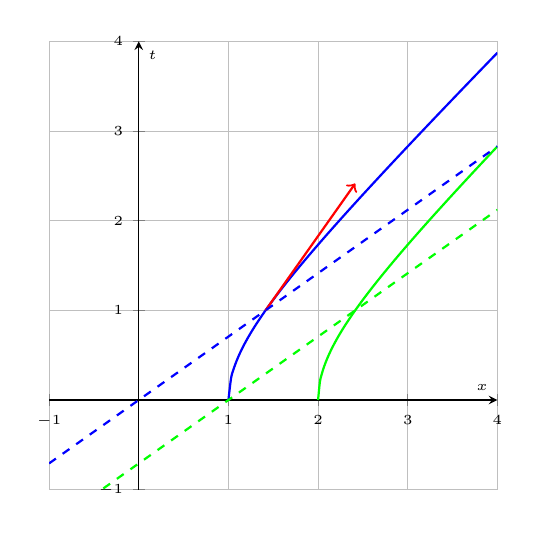
\begin{tikzpicture}
    \begin{axis}[
        axis lines=middle,
        xlabel={$x$},
        ylabel={$t$},
        xlabel style={font=\tiny}, % Makes the x-axis label smaller
        ylabel style={font=\tiny}, 
        xmin=-1, xmax=4,
        ymin=-1, ymax=4,
        grid=both,
        grid style={line width=.1pt, draw=gray!10},
        major grid style={line width=.2pt,draw=gray!50},
        axis equal image,
        legend pos=north west,
        tick label style={font=\tiny}, 
    ]
    % Original hyperbola (positive y values only)
    \addplot[domain=1:4, samples=100, smooth, thick, blue] {sqrt(x^2 - 1)};

    % Shifted hyperbola (positive y values only)
    \addplot[domain=2:4, samples=100, smooth, thick, green] {sqrt((x-1)^2 - 1)};

    % Tangent vector at x=2
    \draw[->, thick, red] (axis cs:{sqrt(2)},1)--++(axis direction cs:1,{sqrt(2)});

    % Calculate slope
    \pgfmathsetmacro{\slope}{1/sqrt(2)}

    % Calculate y-intercept
    \pgfmathsetmacro{\yintercept}{1 - \slope*sqrt(2)}

    % Plot the line
    \draw[thick, blue, dashed] (-1,{\slope*-1 + \yintercept}) -- (4,{\slope*4 + \yintercept}) node[right] {};

    \pgfmathsetmacro{\yinterceptNew}{1 - \slope*(1 + sqrt(2))}

    % Plot the new line
    \draw[thick, green, dashed] (-1,{\slope*-1 + \yinterceptNew}) -- (4,{\slope*4 + \yinterceptNew}) node[right] { };
    \end{axis}
\end{tikzpicture}
\end{document}

